\chapter{Prevalence estimates from other data types}
\label{theory-system_dynamics}
\chapterprecis{Abraham D. Flaxman}

In order to inform age-specific estimates of prevalence with data on
other epidemiological parameters (such as incidence, remission, and
mortality), I now introduce the framework that I call
\emph{integrative systems modeling.}

Integrative systems modeling (ISM) combines a mechanistic model of
process with a statistical model of data.  The foundations of ISM are
best articulated in terms of \emph{system dynamics modeling}, a
discipline that originated in the fields of operations research and
industrial engineering. \cite{forrester_industrial_1961,
  forrester_urban_1969,forrester_world_1973,meadows_thinking_2008}
This type of compartmental modeling is similar to infectious disease
modeling \cite{hethcote_qualitative_1976,andersen_infectious_1991,
  diekmann_mathematical_2000,keeling_modeling_2008,
  vynnycky_infectious_2010} and pharmacokinetic/pharmacodynamic
(PK/PD) modeling
\cite{sheiner_modelling_1972,jacquez_compartmental_1980,yuh_population_1994,
  barrett_saam_1998,jacquez_modeling_1999,atkinson_introduction_2007}

System dynamics modeling is a method to model the behavior of complex
systems in terms of stocks, flows, and feedback loops.  In short,
\emph{stock variables} quantify the amount of some material, mass, or
population in a compartment at a particular moment in time, while
\emph{flow variables} quantify the rate of material moving into, out
of, or between compartments. The scope of applications for system
dynamics is enormous, and once you start thinking of systems in this
way, it may seem that everything can be modeled as stocks and
flows. This method has been applied to the study of complex systems in
economics, politics, environmental science, and a diverse array of
other fields.  \cite{meadows_thinking_2008,jacquez_modeling_1999,
  harte_consider_1988,richardson_feedback_1991,}


Traditionally, there is a delineation between system dynamics modeling
and statistical modeling in the following way: system dynamics aims to
develop a \emph{model of process}, while statistical approaches focus
on developing a \emph{model of data}. Models of process attempt to
explicitly represent the mechanisms behind some system behavior
(deterministically or stochastically), while models of data often
explicitly avoid requiring such a theory. The advantage of using the
system dynamics approach is that it can incorporate structural
assumptions about the system.  However, in many applications, the
systems-dynamics model of process is not connected to data at all.  On
the other hand, in many statistical approaches, the domain-specific
dynamics of the system under study are not incorporated in the model
explicitly, and the data models could benefit from this additional
structure.  Integrative systems modeling is a framework to bring
together a model of process and a model of data for mutual benefit.

\section{A motivating example: population dynamics}

An example will help to make these concepts more concrete.  We begin
with the simplest of compartmental models, a single compartment with
in-flow, out-flow, and no feedback, shown schematically in
Figure~\ref{forward-sim-one-compartment}.

\begin{figure}[h]
\begin{center}
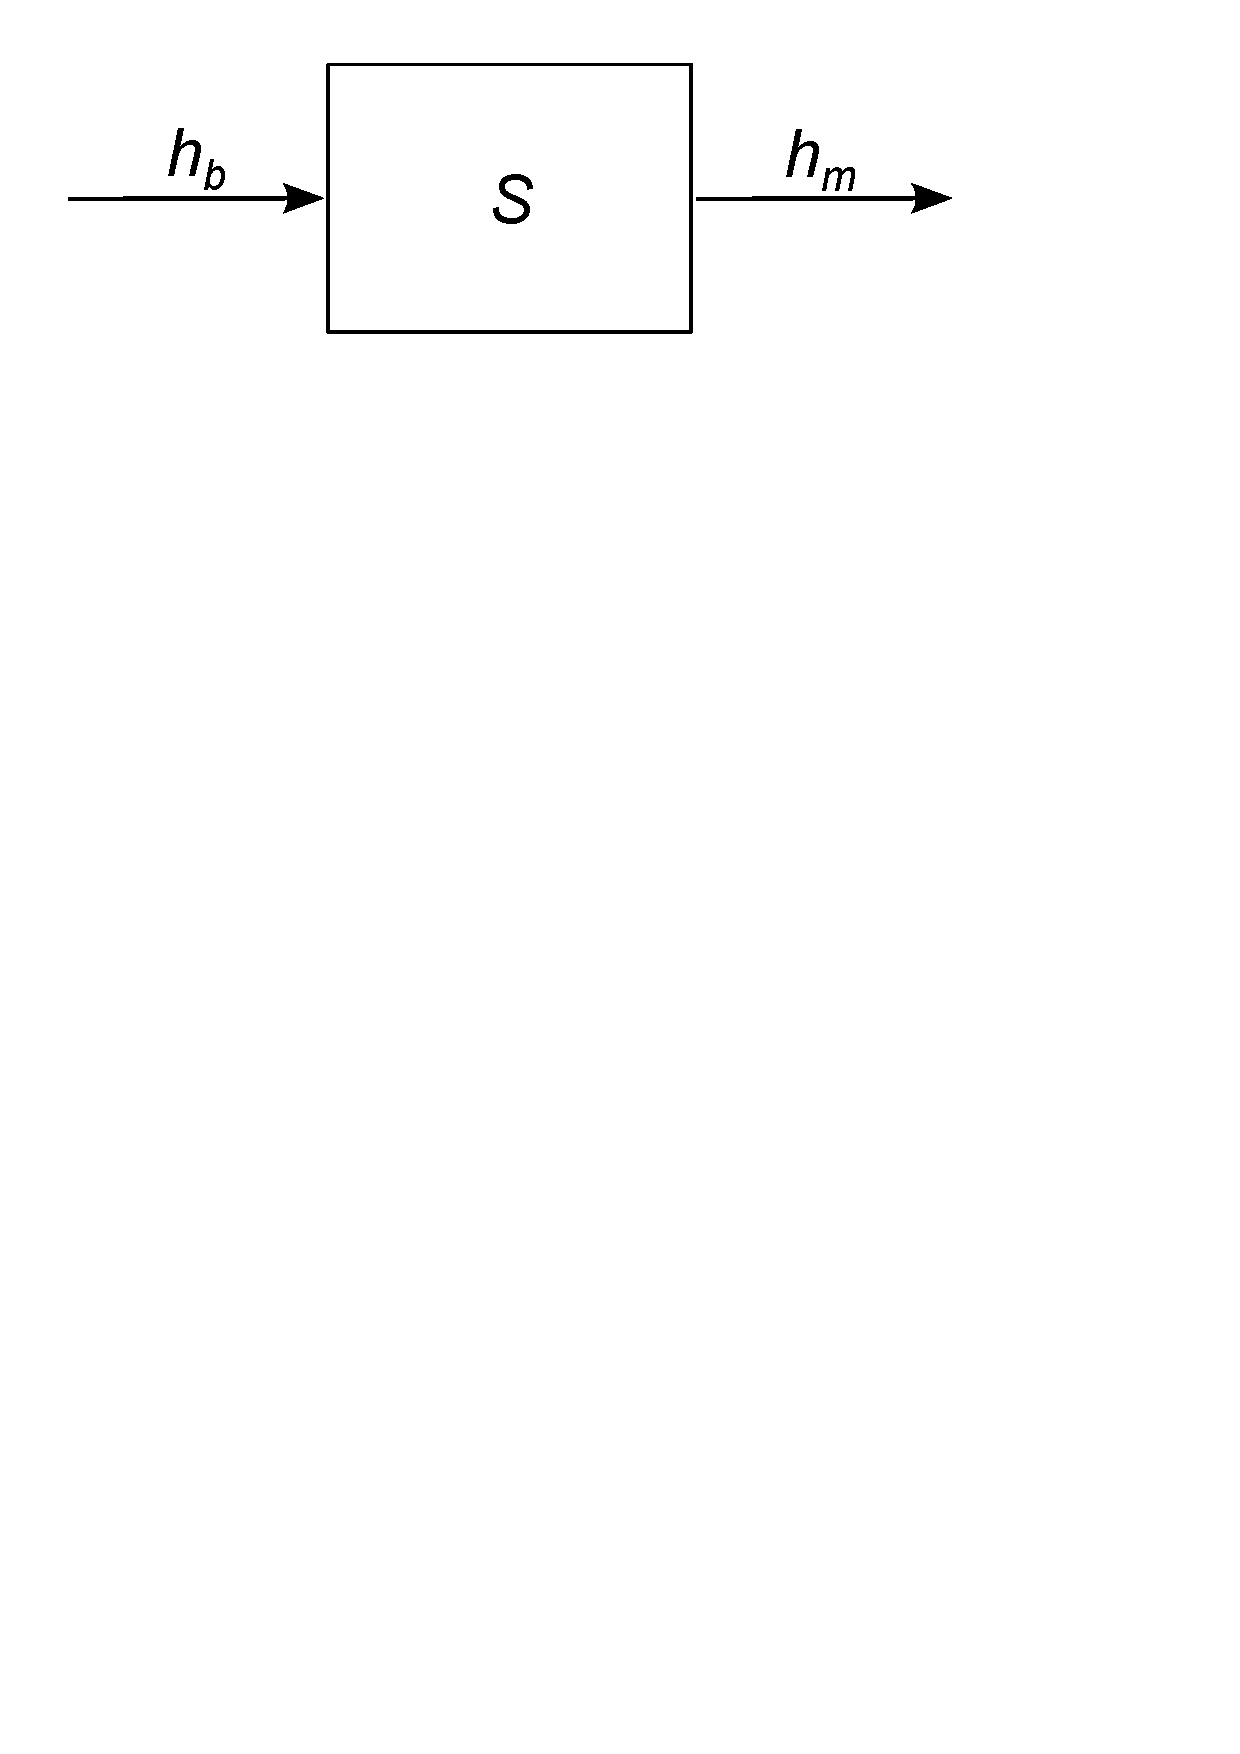
\includegraphics[width=3in]{S.pdf}
\caption{A single compartment model with in-flow $b$ and out-flow $m$
  is one of the simplest examples of a compartmental model. Despite
  its simplicity, it is a useful model of population dynamics.  In
  this application, $b$ represents births, and $m$ represents
  mortality, while $S$ represents the ``stock'' of
  population.}
\label{forward-sim-one-compartment}
\end{center}
\end{figure}


Schematic diagrams of stock-and-flow models such as
Figure~\ref{forward-sim-one-compartment} are useful in understanding
and communicating the structure of a model of process, but they are
incomplete (at least as commonly used in epidemiology; conventions in
PK/PD differ). The full description is represented in the form of a
system of difference equations or differential equations that specify
precisely the relationship between the stocks and flows. The following
differential equation fully specifies the one-compartment model:

\begin{align*}
\frac{dS}{dt}&= b - m\\
b&=h_b S\\
m&=h_m S
\end{align*}

In this equation, the stock $S$ changes continuously, increasing with
birth hazard $h_b$ and decreasing with mortality hazard $h_m$. When
$h_b$ and $h_m$ are constants with respect to time, this differential
equation has a closed-form solution, of $S = S_0 e^{(h_b-h_m)t}$. When
$h_b$ and $h_m$ are not constant with respect to time, the model does
not necessarily have a closed form solution, and many more time trends
are possible for $S$.  Figure~\ref{forward-sim-one-compartment-soln}
shows the time trend of $S$ when $h_b$ and $h_m$ are constant in panel
(a) and when they are changing in panel (b).

\begin{figure}[h]
\begin{center}
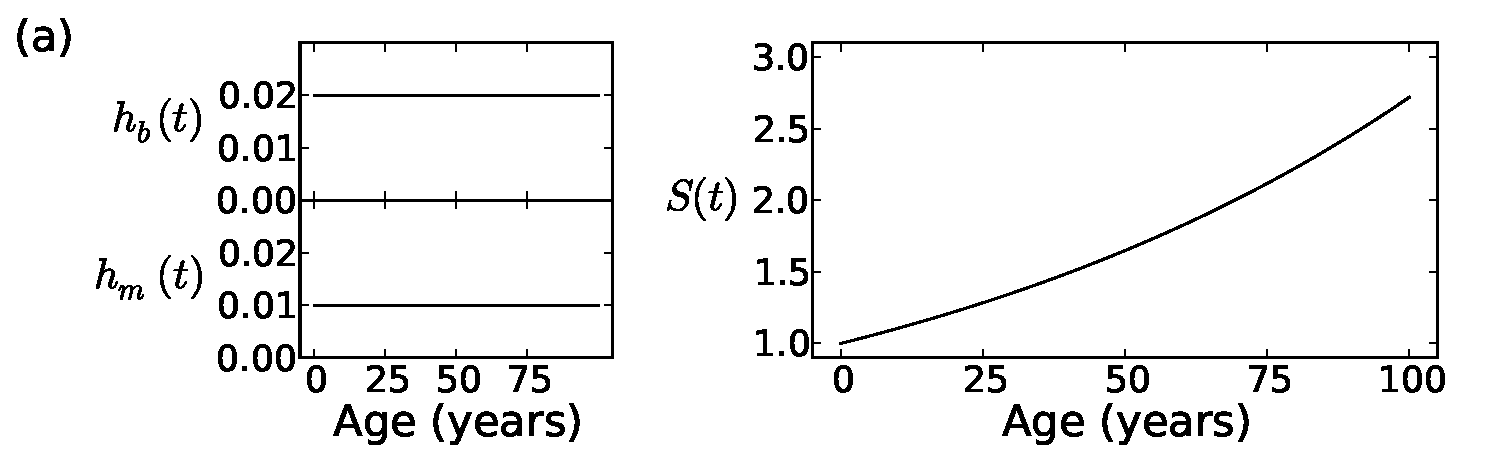
\includegraphics[width=\textwidth]{one_compartment_constant_rate.pdf}
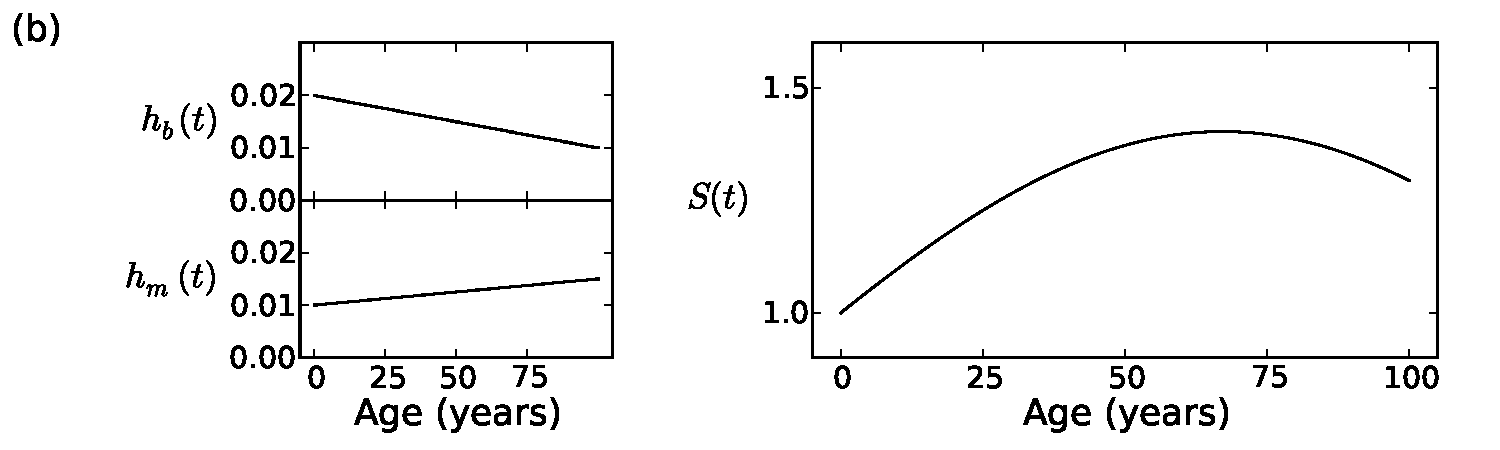
\includegraphics[width=\textwidth]{one_compartment_varying_rate.pdf}
\caption{Stock and flow in a one-compartmental model as a function of
  time. Panel (a) shows the exponentially growing stock when in-flow
  and out-flow hazards are constant with respect to time, and the in-flow
  exceeds the out-flow.  Panel (b) shows the non-monotonic change
  in stock with respect to time in a system where the in-flow hazard is
  decreasing as a function of time and the out-flow hazard is
  increasing.}
\label{forward-sim-one-compartment-soln}
\end{center}
\end{figure}


%% \section{Related work}

%% The field of system dynamics modeling, from which ISM borrows terminology and
%% inspiration, developed in the management sciences. An early application was
%% in explaining employment cycles at a large company's appliance plants
%% \cite{forrester_counterintuitive_1971}. The prevailing theory of the
%% time was that hiring and firing cycles followed general economic
%% cycles. However, a compartmental model of the system underlying the
%% appliance business showed that the employment cycles arose from
%% feedback loops inherent to the company's internal structure and could be
%% smoothed out by modifying conditions entirely under the company's
%% control. This first application demonstrates a major theme in system
%% dynamics modeling. In complex systems, determinants of system behavior
%% considered individually may be insufficient to predict the behavior of
%% that system. The most important behavior in a complex system arises
%% out of interactions and feedback between processes in that
%% system---this is also the case in disease modeling where the dynamic
%% nature of the disease process should be taken into account. The
%% information contained in modeling the entire disease
%% process---including incidence, remission, and mortality---for a given
%% disease can exceed the information contained in separate analyses of
%% that disease's mortality, incidence, and remission separately. There
%% is increasing interest in applying system dynamics to solve a number
%% of diverse health issues that require a model with sufficient
%% complexity to incorporate multi-causal relationships. Fields such as
%% pharmacology, epidemiology, and public health have applied
%% compartmental models to tackle a range of interesting modeling
%% challenges.

%% Pharmacokinetic and pharmacodynamic (PK/PD) modeling, a subdiscipline
%% of pharmacology, developed an approach to compartmental modeling in
%% tandem with system dynamics modeling largely independently.  However,
%% the mathematics behind the models of process are extremely
%% similar. The compartments in PK/PD models represent organs and other
%% physical systems in the body, and stocks represent the quantities of
%% pharmacologically relevant compounds in these compartments.  The flows
%% model the process of the drug of interest being metabolized or
%% otherwise passing through the subject. Mathematically, these models
%% have precise parallels to the stock-and-flow models developed for
%% supply chain analysis. For instance, in one recent application,
%% experiment researchers used a compartmental model approach to
%% understand glucose kinetics.\cite{Gastaldelli_Glucose_1997} They found
%% that a three-compartment model where two compartments correspond to
%% peripheral pools exchanging plasma at different rates with a central
%% pool best represented the physiology of glucose kinetics in their test
%% subjects (in this case, a sample of seven sheep). This particular
%% model structure has arisen several times in applications in
%% pharmacokinetics, and is called the mammillary model. In another
%% experiment, researchers modeled the kinetics of epsilon-aminocaproic
%% acid (EACA) in six human subjects. EACA is a compound used to control
%% hemorrhage in patients with bleeding problems. The PK/PD researchers
%% developed a multicompartmental model, where EACA was infused in a
%% central compartment, distributed to fast- and slow-excreting
%% peripheral compartments, and cleared by two compartments, one
%% representing renal excretion of the drug, and another representing
%% nonrenal excretion.\cite{Frederiksen_Kinetics_1984} In both of these
%% examples and in general practice in pharmacokinetics, the
%% compartmental model of process is connected to a statistical model of
%% data. This connection is the central idea of integrative systems
%% modeling, and will be developed in detail in later chapters.



%% One area in which public health has a long tradition of compartmental
%% and system dynamics modeling is in infectious
%% disease.\cite{Anderson_Infectious_1991, Hethcote_Qualitative_1976,
%%   Blower Hypercube sampling} For example, the
%% Susceptible-Infective-Recovered (SIR) compartmental model, which was
%% discussed in Chapter~\ref{intro-sim}. This basic model has been
%% extended in a variety of ways in order to model increasingly more
%% complex infectious disease dynamics. For instance, in one study
%% Nagelkerke and colleagues modeled the impact of a range of
%% interventions targeted at preventing transmission of HIV/AIDS
%% epidemics \cite{ref}. They estimated impact using a compartmental
%% model where the population moved from an ``Uninfected'' compartment to
%% either treated or untreated ``Infected'' compartments to an ``AIDS''
%% compartment to a ``Death from AIDS'' compartment.

%% Another example that makes an explicit connection between
%% epidemiological modeling and system dynamics is the recent work by
%% Kershenobich and colleagues, who applied a systems approach to
%% forecasting the prevalence of hepatitis C. They developed a
%% compartmental model tracking incidence, diagnosis, and treatment of the
%% disease. For the incident population in the model, an individual moves
%% from an acute phase (which lasts for six months) to a chronic phase,
%% unless that individual is spontaneously cleared of the disease, is
%% treated and cured, or dies. For the prevalent population in the model,
%% an individual moves from viraemic to nonviraemic, dies, or gets
%% treated and cured. Separate models were also used to estimate the
%% mortality rate in different countries based on age, liver-related
%% deaths due to hepatitis C infection, and percent of the population
%% infected by injection drug use. Sensitivity analyses were conducted
%% by running the model for a number of input scenarios.  This model allowed the authors to predict the future trend of hepatitis C prevalence and quantify uncertainty with missing and inaccurate data in very heterogeneous populations.  Without this approach, more modeling assumptions must be made and the relationship between assumptions and results are less clearly understood. \cite{kershenobich_applying_2011}

%% Health systems are particularly complex, with many actors and many
%% feedback loops providing a large supply of systems modeling
%% opportunities. The health of a population is affected by a combination
%% of biological, economic, demographic, and political forces, and all of
%% these spheres interact in a unexpected ways. Since the 1970s, system
%% dynamics models have been applied to model these various forces in
%% order to advance our understanding of population health \cite{refs}
%% from
%% \url{http://www.systemswiki.org/images/f/f5/SD_background_for_public_health_%284.11.05%29.pdf}. The
%%   topics addressed have included disease epidemiology, substance
%%   abuse epidemiology, patient flows in emergency care, health care
%%   capacity and delivery, and interactions between health care and
%%   disease epidemiology. A systems approach is often required, because
%%   isolating one part of a public health problem and then addressing
%%   that may in fact adversely affect other parts of the system. For
%%   instance, low tar/nicotine cigarettes were developed to address one
%%   part of the burden of disease caused by tobacco consumption, but
%%   consumer behavior was not taken into account. Consumers tended to
%%   take longer, more frequent drags and thus negated the benefit of the
%%   low tar/nicotine content \cite{Sterman_Learning_2006}. A systems
%%   approach would seek to simultaneously account for both the effect of
%%   the tobacco product on the consumer and the consumer's behavior. In
%%   the context of modeling the progression of a disease through a
%%   population, a model that seems to describe infection dynamics
%%   accurately may conflict with data on remission or fatality. Only by
%%   modeling the three together can the analyst get the most accurate
%%   and consistent estimates.

%% In another health system-focused example, Flaxman and colleagues
%% developed a stock-and-flow model to synthesize data on the
%% availability and distribution of insecticide-treated bednets (ITNs)
%% and to predict the proportion of households that owned an ITN. This
%% analysis employed a Bayesian approach to estimate the parameters of
%% the compartmental model that describe the process of ITNs moving from
%% warehouses and other storage facilities into the household and
%% possibly getting discarded by the households or lost in the
%% distribution process.  This approach is commonly used by
%% pharmaceutical firms to track their product.

%% These examples provide a basic understanding of the myriad uses for
%% systems dynamics modeling. The following chapters will detail how
%% these same ideas can be applied to a model-based metaregression tool
%% for disease modeling.




%% TK connection to the references cited in this NIH RFP for systems modeling
%% \url{http://grants.nih.gov/grants/guide/pa-files/PAR-08-224.html}
%% \url{http://ajph.aphapublications.org/cgi/content/full/96/3/452}
%% \url{http://www.systemswiki.org/index.php?title=Health_System_Dynamics_References}




I will now focus on the specific application that is crucial to
model-based meta-regression: the system dynamics of a disease moving
through a population, with flows that vary as a function of age.

\section{System dynamics model of disease in a population}
\label{sys-dynamics}
The key to combining data of different types is a two-compartment
system dynamics model of process. The compartments contain the
population susceptible to the disease (stock $S$, for ``susceptible'')
and the population with the condition (stock $C$, for
``condition''). The population moves between these compartments
following the arrows shown in
Figure~\ref{forward-sim-two-compartment}, transitioning from $S$ to
$C$ with incidence hazard $h_i$, and from $C$ back to $S$ with
remission hazard $h_r$. The susceptible population flows out of the
system with background mortality hazard $h_m$, and the with-condition
population flows out of the system with with-condition mortality
hazard $h_{m_\with} = h_m+h_f$.  Here $h_f$ represents the ``excess
mortality hazard'' for individuals with the condition over individuals
without the condition.

\begin{figure}[h]
\begin{center}
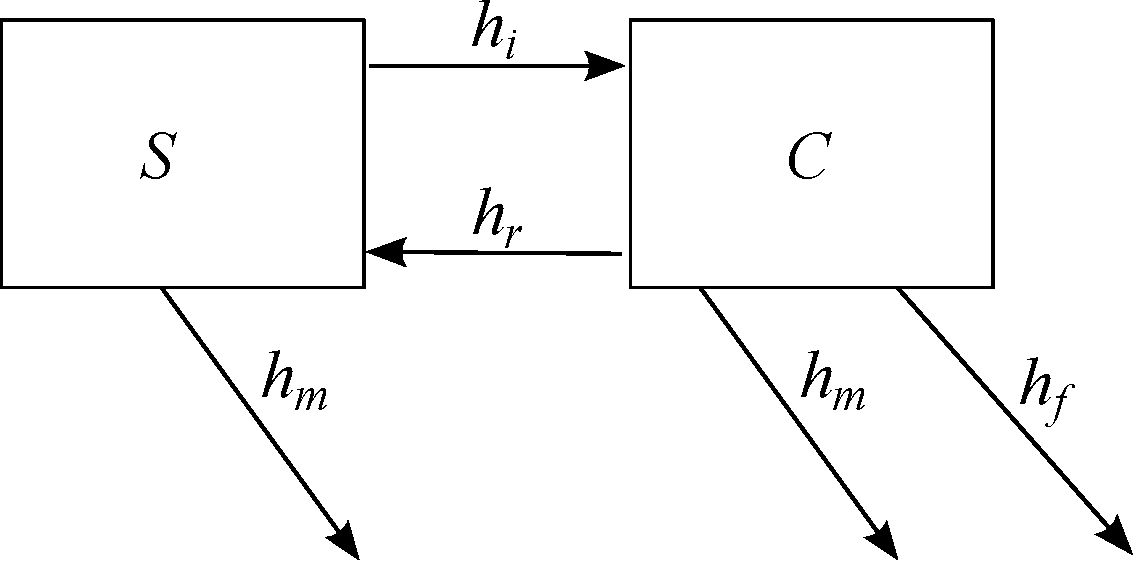
\includegraphics[width=5in]{SC.pdf}
\caption{The two-compartment model of process for disease in a
  population, around which the meta-regression framework is
  built. Compartment $S$ contains the population susceptible to the
  disease and compartment $C$ contains the population with the
  condition. Individuals move from $S$ to $C$ with incidence hazard $h_i$,
  and from $C$ to $S$ with remission hazard $h_r$. The susceptible
  population flows out of the system with without-condition mortality
  hazard $h_m$, and the with-condition population flows out of the system
  with with-condition mortality hazard $h_m+h_f$, where $h_f$ is the excess
  mortality hazard, representing quantitatively the increase in
  mortality for individuals with the condition.}
\label{forward-sim-two-compartment}
\end{center}
\end{figure}


This ``model of process'' looks deceptively simple, and compared to
the complex systems often developed in infectious disease modeling it
\emph{is} quite simple.  However, it more flexible than it appears at
first glance.  All of the parameters of the model are functions of
age and time, which permits enough flexibility to match well the
myriad of available data about the descriptive epidemiology of
disease.  In the coming sections, we will connect this model of
process to an appropriately complex model of data, and together they
will provide our integrative systems model for model-based
meta-regression.

As mentioned in the previous section, a schematic depiction of a
compartmental model, such as Figure~\ref{forward-sim-two-compartment},
is not a complete description of the system dynamics.  To specify them
completely I now turn to a system of differential equations,
which correspond to the stocks and flows above, and more precisely
represent their relationship as a function of time and age:
\begin{align*}
\frac{\d }{\d \t} S(a+\tau,t+\tau) &= -(h_i + h_m)S + h_rC,\\
\frac{\d}{\d \t} C(a+\tau,t+\tau) &= h_iS - (h_r + h_m + h_f)C,\\
\end{align*}
where $S,C,h_i,h_r,h_m,$ and $h_f$ are shorthand for the following functions of age and time:
\begin{align*}
S &= S(a,t) = \text{stock of ``susceptibles''},\\
C &= C(a,t) = \text{stock of ``with condition''},\\[.1in]
h_i &= h_i(a,t) = \text{incidence hazard for susceptibles},\\
h_r &= h_r(a,t) = \text{remission hazard for individuals with condition},\\
h_m &= h_m(a,t) = \text{without-condition mortality hazard for susceptible},\\
h_f &= h_f(a,t) = \text{excess-mortality hazard for individuals with
condition}.
\end{align*}
In general, all of these quantities are functions of both age $a$ and
time $t$.

At this point in developing the model of process it is valuable to
pause and consider what descriptive epidemiological data may be
collected in a systematic review of the literature and other sources,
and how they can correspond to the stocks and flows in the model,
through a suitable model of data.

For certain especially infectious diseases, cases identified in the
health system are required to be promptly reported to the WHO; for
example, the incidence of tuberculosis.  This yields data on disease
incidence rates (which is not age-specific, i.e., crude incidence rate
over all ages).  All caveats about case reports and health system
access are deferred for future discussion, but the number of cases per
year divided by the midyear population provides an approximate
measurement of the incidence hazard $h_i$ in the figure above.

Often it is prevalence that is directly measured, for example through
a household or telephone survey.  This sort of research provides
measurements of the form $k$ out of $n$ respondents tested positive
for the condition (or said that they had the condition). simple
division or some more complicated survey analysis method then yields a
measurement of the ratio of compartments in the stock and flow model
above, i.e., prevalence is equal to $C/(S+C)$.  Often this
information will be stratified by age and/or sex, and for many
important diseases, the prevalence level will vary by orders of
magnitude over the age range of the population.

There is another sort of study that is often available, one that
measures the relative mortality ratio of a disease, meaning the
mortality rate in people with the disease and without the disease, and
reports the ratio (sometime called the relative risk).  This
corresponds to a ratio of hazards in the model above, $(h_m+h_f) /
h_m$.  Unfortunately, $h_f$ is rarely measured directly, but the
with-condition mortality hazard is sometimes reported instead of
relative mortality risk, which can be represented as $h_{m_{\with}} =
h_m+h_f$.

The all-cause mortality for a population can also be
derived from the model, as $h_{m_\all} + \frac{C}{S+C}h_f$.  The quantity
$\frac{C}{S+C}h_f$ is important in its own right, because for
conditions that are unambiguously coded as the cause of death on death
certificates, the population-level cause-specific mortality rate
(i.e., the fraction of death certificates with this cause coded as the
underlying cause of death) is approximately equal to this
population-level cause-specific mortality rate.  Even for conditions
where the death certificates are not likely to be coded to this cause
for all deaths (e.g.,~diabetes), the population-level cause-specific
mortality rate is a lower bound on $\frac{C}{S+C}h_f$, which can still
provide useful information.

There is an important distinction between the hazards $h_{m_{\with}}$
and $\frac{C}{S+C}h_f$, and that is the population to which they
apply. $h_{m_{\with}}$ applies \emph{only} to the with-condition
population, while $\frac{C}{S+C}h_f$ applies to the general
population, including both those with and without the condition.
$h_{m_{\with}}$ can be measured by following a cohort of individuals
with the condition over time, while $\frac{C}{S+C}h_f$ can (sometimes)
be measured by looking at deaths due to the condition in the general
population.

Remission and duration studies, in which individuals with the disease are
tracked over time to estimate how long the disease persists, provide
yet another measurement that corresponds to parameters in this model
(in the case of remission) or a quantity that can be derived from the
model parameters (in the case of duration).

Representing mean duration of disease, i.e., the expected time an
individual spends in compartment $C$ before leaving, is a relatively
involved calculation, included here for completeness:
\begin{align*}
\text{duration}(a, t) &
= \int_{\tau = 0}^\infty e^{-\left(h_r(a+\tau, t+\tau) + h_f(a+\tau, t+\tau) + h_m(a+\tau, t+\tau)\right) \tau}\d \tau
\end{align*}
This integral can be simplified considerably for certain special
cases.  For example, if the remission hazard is constant as a function
of age and time, and the mortality hazards $h_m$ and $h_f$ are small, the duration
simplifies to $\int_{\tau \geq 0} e^{-h_r\tau}\d \tau =
\frac{1}{h_r}.$ This justifies the approximation that remission rate is
nearly equal to one over duration in acute conditions.

The data available for these parameters varies widely between the
diseases that have been analyzed in the GBD 2010 Study. Some diseases
have many and more data, while others have only prevalence or only
incidence and not much of that. These gaps and the bridges between
what we know and what we want to know will be explored in theory and
practice in several later sections of this book.

With this detour through potentially available data in mind, it is now
instructive to return to the more challenging elements of the
compartmental model. Conceptually, it is excess mortality hazard $h_f$
that has proven hardest to explain and to understand. This is because
in most, if not all, applications, $h_f$ is a latent variable,
unobservable through most any epidemiological study. Perhaps it would
be clearer to talk about the with-condition mortality hazard, which at
least can be measured through a cohort study, and may be more familiar
to the doctor or epidemiologist. With-condition mortality is not
represented directly in the model, but can be derived as
$h_{m_{\with}} = h_m+h_f$.

There are large differences in disease parameters such as incidence
and prevalence as a function of age, and it is essential for a model
to take this into account.  Congenital abnormalities all have a birth
prevalence, while important diseases such as dementia and Alzheimer's
disease have effectively zero prevalence in the young and
dramatically increasing incidence and prevalence at older
ages. Furthermore, the incidence and prevalence of disease, as well as
the remission and excess-mortality hazards, change over time due to
shifts in population, changes in prevention or treatment, and changes
in care. And the interdependence between these factors is complex, but
unignorable: today's population of 50-year-olds will be next year's
51-year-olds.

For these reasons, a system of partial differential equations
describing the change in the size of the compartments as a function of
age and time provides a sufficiently rich theoretical framework for
the model of process.  In this formulation, the incidence, remission,
without-condition mortality, and excess mortality hazards are all
functions of time and age, and the initial conditions for the stock of
susceptible and with-condition population at age zero are functions of
time.

\section{Endemic equilibrium}
\label{theory-forward_sim-compartmental_model-simplying_assumptions}

The full model above is often more complex than can be supported by
available data, which is usually very sparse and very noisy.  In order
to simplify the modeling procedure and reduce the computational challenge
of estimation, I often assume that the disease parameters are not changing
substantially with respect to time. To be precise, this is the assumption
that the partial derivative of all stocks and all flows with respect
to time is zero:
\[
\frac{\partial S}{\partial t}
=
\frac{\partial C}{\partial t}
=
\frac{\partial h_i}{\partial t}
=
\frac{\partial h_r}{\partial t}
=
\frac{\partial h_m}{\partial t}
=
\frac{\partial h_f}{\partial t}
=
0.
\]

Although the primary use of this model is for inference of model
parameters (sometimes called the ``inverse problem''), it is
instructive to apply it to the ``forward problem'' to show how hazards on incidence,
remission, and excess mortality produce different prevalence
curves. The next section explores this forward simulation through a
series of examples to develop an intuition around how consistency
forces interrelationships between prevalence, incidence, remission,
and mortality.


\section{Forward simulation examples}

This section begins with a classic example from the history of generic
disease modeling, the hypothetical example used in describing DisMod
in the first GBD study.\cite{harvard_school_of_public_health.;world_health_organization.;world_bank._global_1996}
The incidence hazard increases linearly from age 0 to
100, and the remission and excess mortality hazards are constant with
respect to age.  Using all-cause mortality data from Southern sub-Saharan
Africa, and a birth prevalence of zero specifies
the forward simulation, producing the outputs shown in
Figure~\ref{forward-sim-ex1}.

\begin{figure}[htb]
\begin{center}
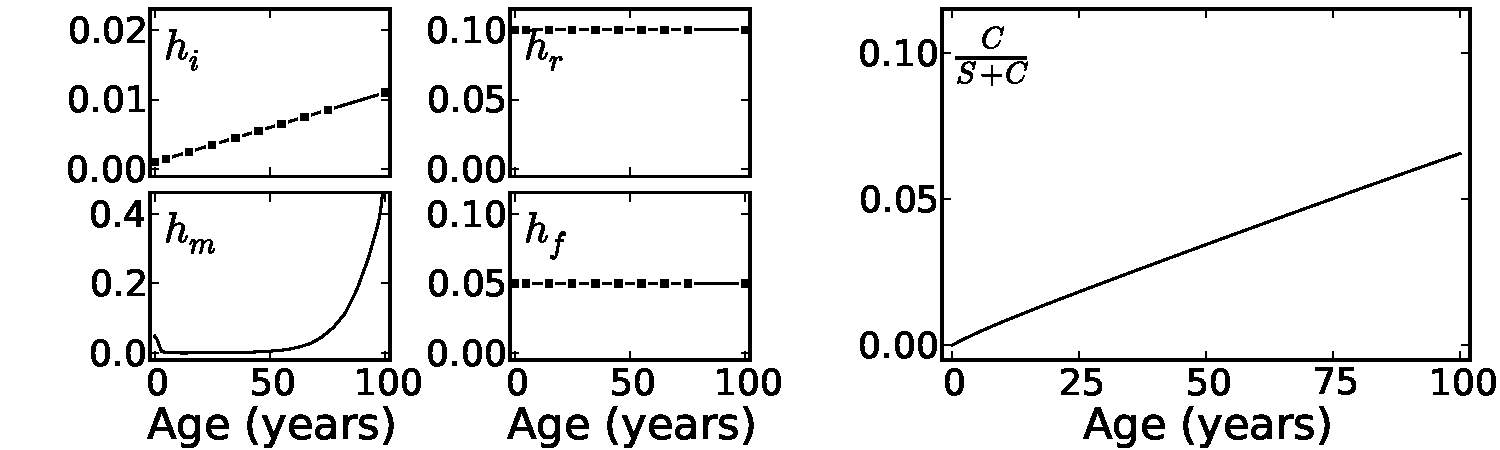
\includegraphics[width=\textwidth]{initial.pdf}
\caption{Consistent disease parameters for a condition where incidence
  ($h_i$) increases linearly as a function of age, while remission
  ($h_r$) and excess mortality ($h_f$) hazards are constant. The
  background mortality ($h_m$) has an age-specific hazard that follows
  all-cause mortality for females in the sub-Saharan, Southern region
  in 1990. For a condition with prevalence of zero at age $0$, these
  hazards lead to a nearly linear increase as a function of age.}
\label{forward-sim-ex1}
\end{center}
\end{figure}

When I change the age pattern of excess mortality to also be linearly
increasing as a function of age, the prevalence curve
becomes more clearly nonlinear, showing a condition that increases in
prevalence quickly in young age groups but slower in older
ages. Figure~\ref{forward-sim-ex2}, panel (a) shows the results
of this change.

Although the prevalence age pattern is largely determined by the
remission, incidence, and mortality hazards, the birth prevalence can
also change the shape
dramatically. Figure~\ref{forward-sim-ex2}, panel (b)
shows the results of the same remission, incidence, and mortality
hazards as in panel (a), but with a birth prevalence of 1.5\%.

\begin{figure}[htb]
\begin{center}
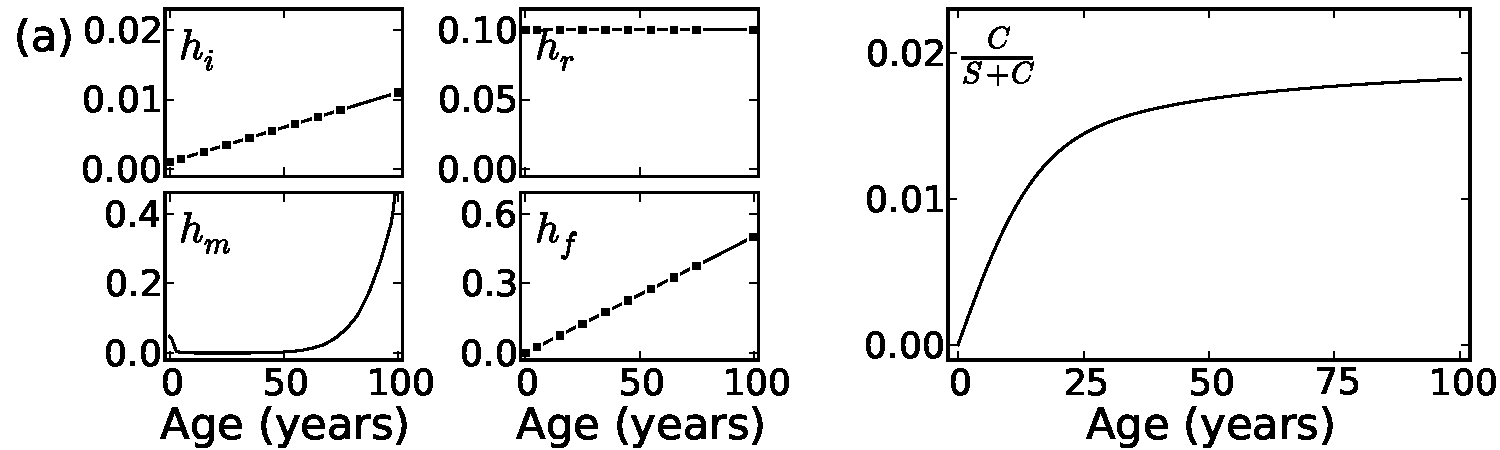
\includegraphics[width=\textwidth]{more-excess-mortality.pdf}
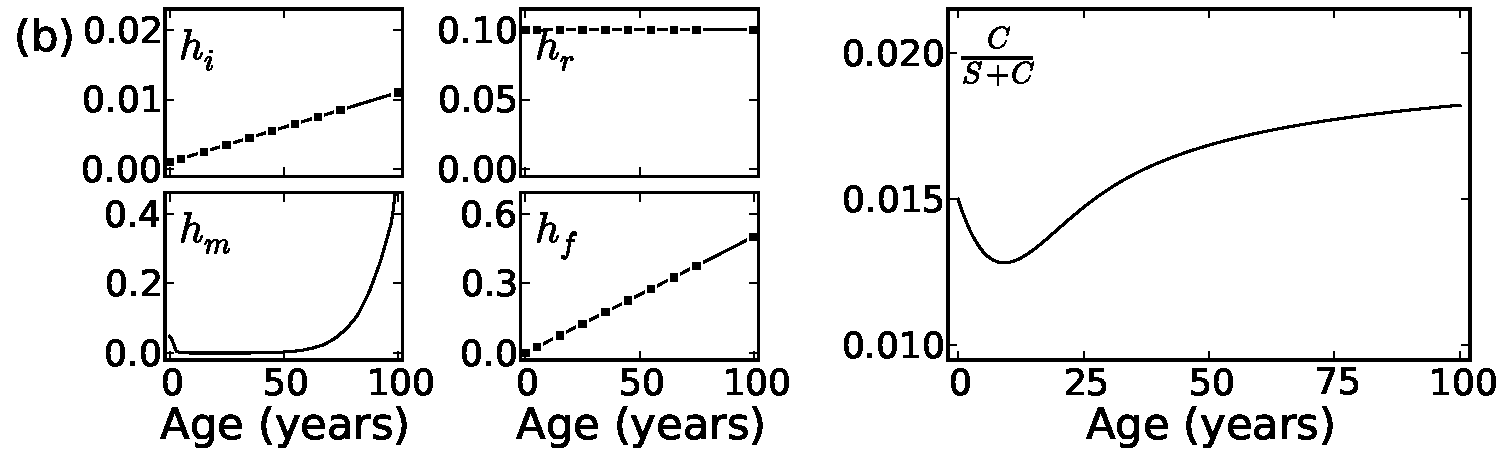
\includegraphics[width=\textwidth]{birth-prevalence.pdf}

\caption{Consistent disease parameters for a condition where incidence
  ($h_i$) and excess mortality ($h_f$) both increase linearly as a
  function of age while remission ($h_r$) is constant. The background
  mortality ($h_m$) has an age-specific hazard corresponding to females in
  the Southern sub-Saharan Africa region in 1990. Panel (a) shows that for a condition
  with prevalence of zero at age $0$, these hazards drive a prevalence
  age pattern which increases quickly in younger age groups and
  more slowly in older age groups. Panel (b) shows that for a condition with prevalence of
  1.5\% at age $0$, these rates yield a prevalence age pattern which is
  highly nonlinear, dipping to a minimum of 1.3\% at age 9, and then
  increasing back up to 1.8\% at the oldest ages.
}
\label{forward-sim-ex2}
\end{center}
\end{figure}


To summarize, this series of figures has shown the intuitive and
less-than-intuitive way that the levels and age patterns of different
epidemiological parameters must be interrelated to satisfy the
fundamental equations of population health (when disease hazards for
each age are changing negligibly slowly as a function of time).

Figure~\ref{forward-sim-ex3} is designed to continue building familiarity with the
features of consistent disease modeling by selecting age patterns for
certain hazards based on schematic models of a variety of diseases.  For
example, for a disorder like depression, for which there is primarily
incidence in early adulthood, high remission hazard, and low excess
mortality, the consistency conditions produce a prevalence age pattern
that peaks at age 25, as shown in panel~(a).
For a congenital disorder, like Down Syndrome, with birth
prevalence, no incidence after birth, no remission, and substantial
mortality, the consistent prevalence age pattern is shown in
panel~(b).
For a disorder that affects the elderly, like Parkinson's Disease, the
consistent age patterns for mortality, incidence, remission, and
prevalence could look roughly like the age-specific rates shown in
panel~(c).
And for disorders related to reproductive health, like premenstrual
syndrome, with zero excess mortality, incidence during ages 15-60, and
remission that increases substantially at age 55, the consistent age
patterns could look like those shown in
panel~(d).
To conclude this series of plots, I've included an ``incidence impulse
response'' example, showing the prevalence produced to be consistent
with an incidence pattern that is only nonzero for a single age
group. This is the content of
panel~(e).


\begin{figure}
\begin{center}
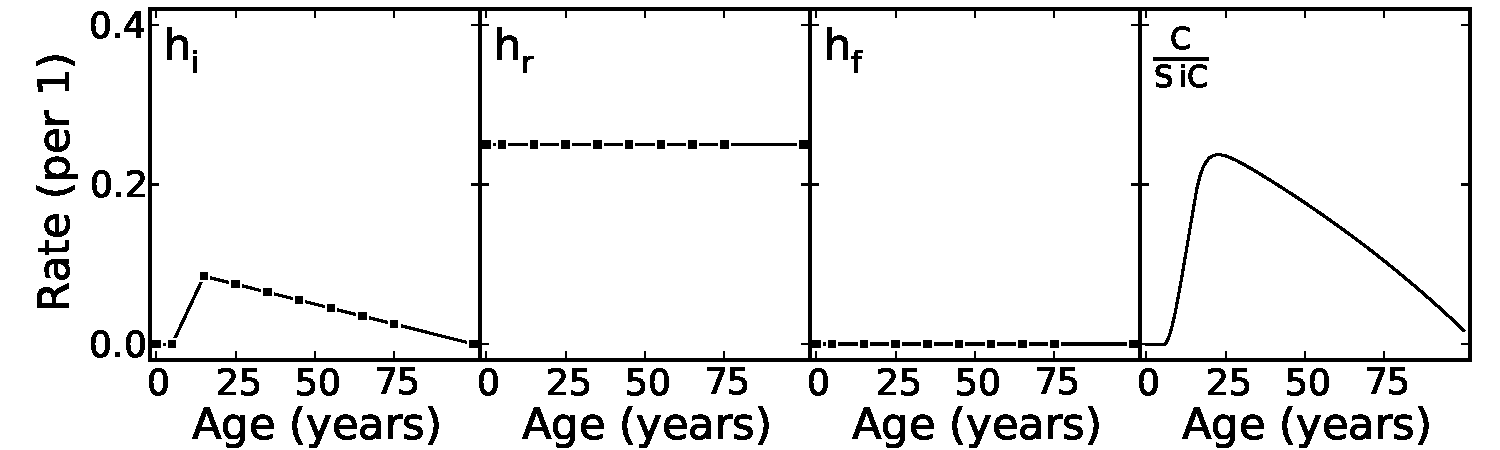
\includegraphics[width=\textwidth]{forward-sim-mental.pdf}
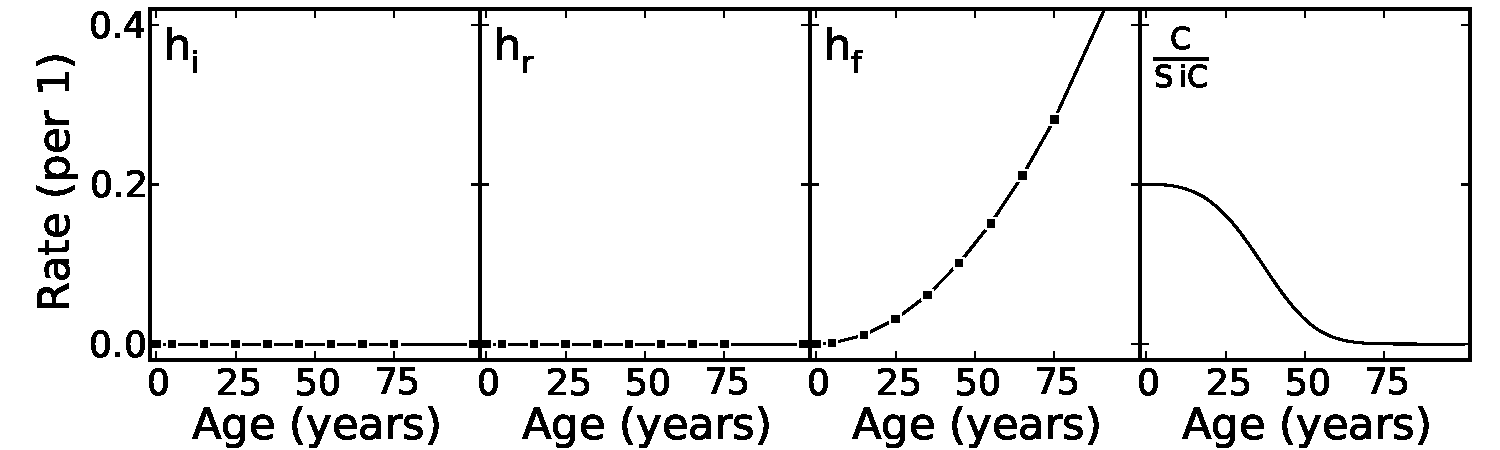
\includegraphics[width=\textwidth]{forward-sim-congenital.pdf}
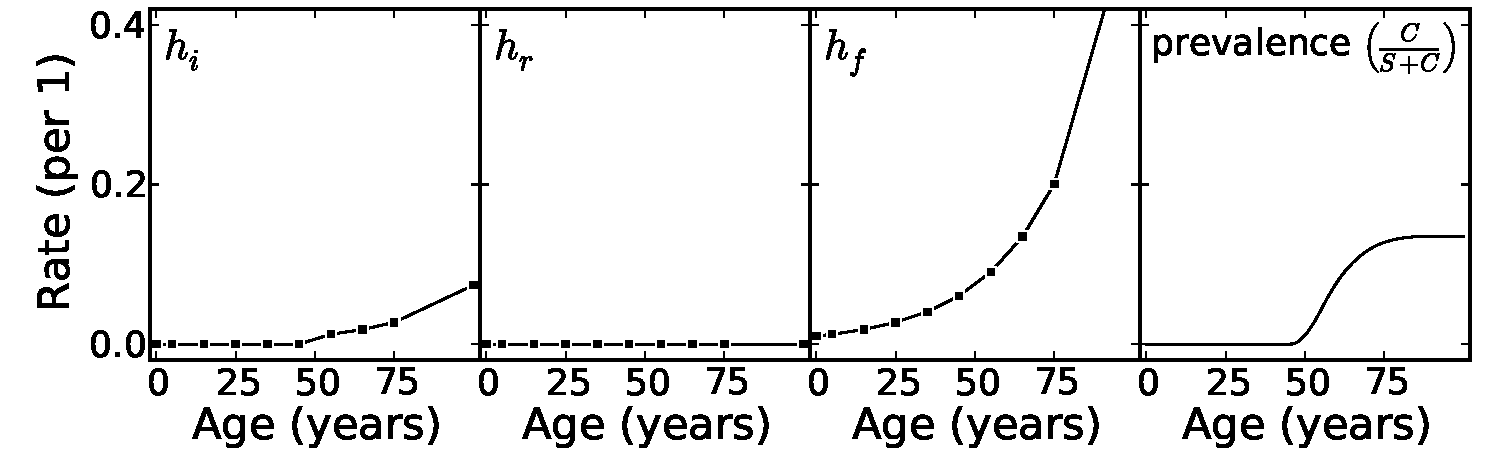
\includegraphics[width=\textwidth]{forward-sim-old_age.pdf}
\caption{ (a) In a disorder like depression, the excess mortality rate is
  very low, and the remission rate is substantial.  In this case, the
  age-pattern of the incidence rate drives the age pattern of
  prevalence in a slightly nonlinear fashion, where the age pattern
  of prevalence is a ``smoothed'' copy of the incidence age pattern.
(b) For a condition acquired before or during birth, such as
  Down Syndrome, incidence and remission are often very low, while
  excess mortality may increase with age.  This leads to prevalence
  that decreases as a function of age.
(c) For a condition that occurs in older age groups, such as
  Parkinson's Disease, the age-specific rates may look like these,
  where increasing incidence drives increasing prevalence in older age
  groups, but the countervailing force of increasing excess mortality
  causes the prevalence increase to level out or even decline the at
  oldest ages.
}
\label{forward-sim-ex3}
\end{center}
\end{figure}

\begin{figure}
\begin{center}
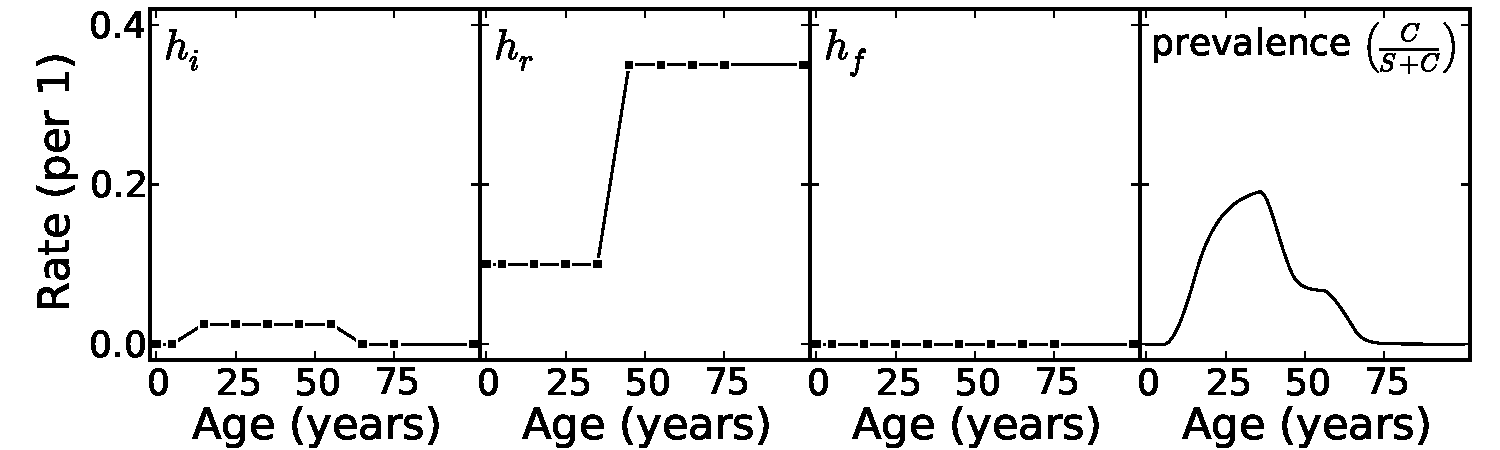
\includegraphics[width=\textwidth]{forward-sim-reproductive.pdf}
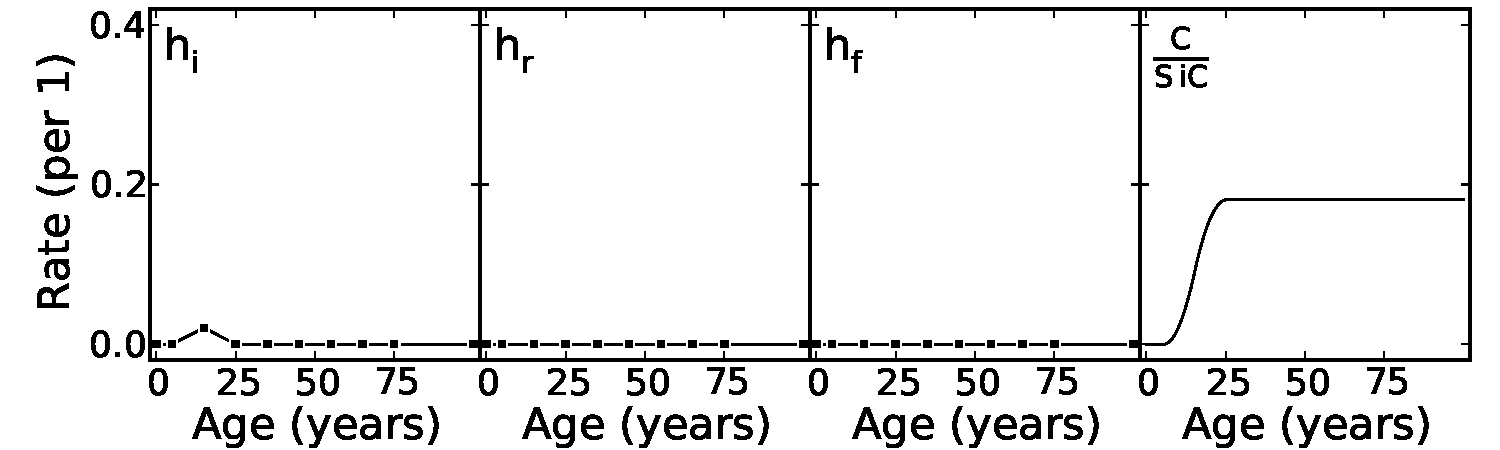
\includegraphics[width=\textwidth]{forward-sim-incidence_pulse.pdf}
\caption{(d) For a condition related to reproductive health, like
  premenstrual syndrome, the age-specific rates may look like these,
  where incidence is nonzero during reproductive ages and zero in
  the very young and old, and remission increases steeply at age
  50. This age pattern, with some shifts in age groups, is also similar
  to that seen in data on substance dependence.
(e) The results of an ``incidence pulse'' show how the system
  responds to a condition with no excess mortality and no remission
  that is incident only for a limited number of young ages.  This
  incidence age function produces a sigmoidal age pattern in
  prevalence, which transitions from zero to nonzero during the ages
  that incidence is nonzero, and then stays at this value for all
  older ages.}
\label{forward-sim-ex3b}
\end{center}
\end{figure}


